\chapter{Extending the system}
\label{ch:extending}

In this section we show how we design our system to be extensible
in terms of adding new matching algorithms, also using existing
shared methods, or sharing new methods.

\section{Matching algorithms inheritance}

\begin{figure}[H]
\centering
\captionsetup{justification=centering}
\makebox[\textwidth][c]{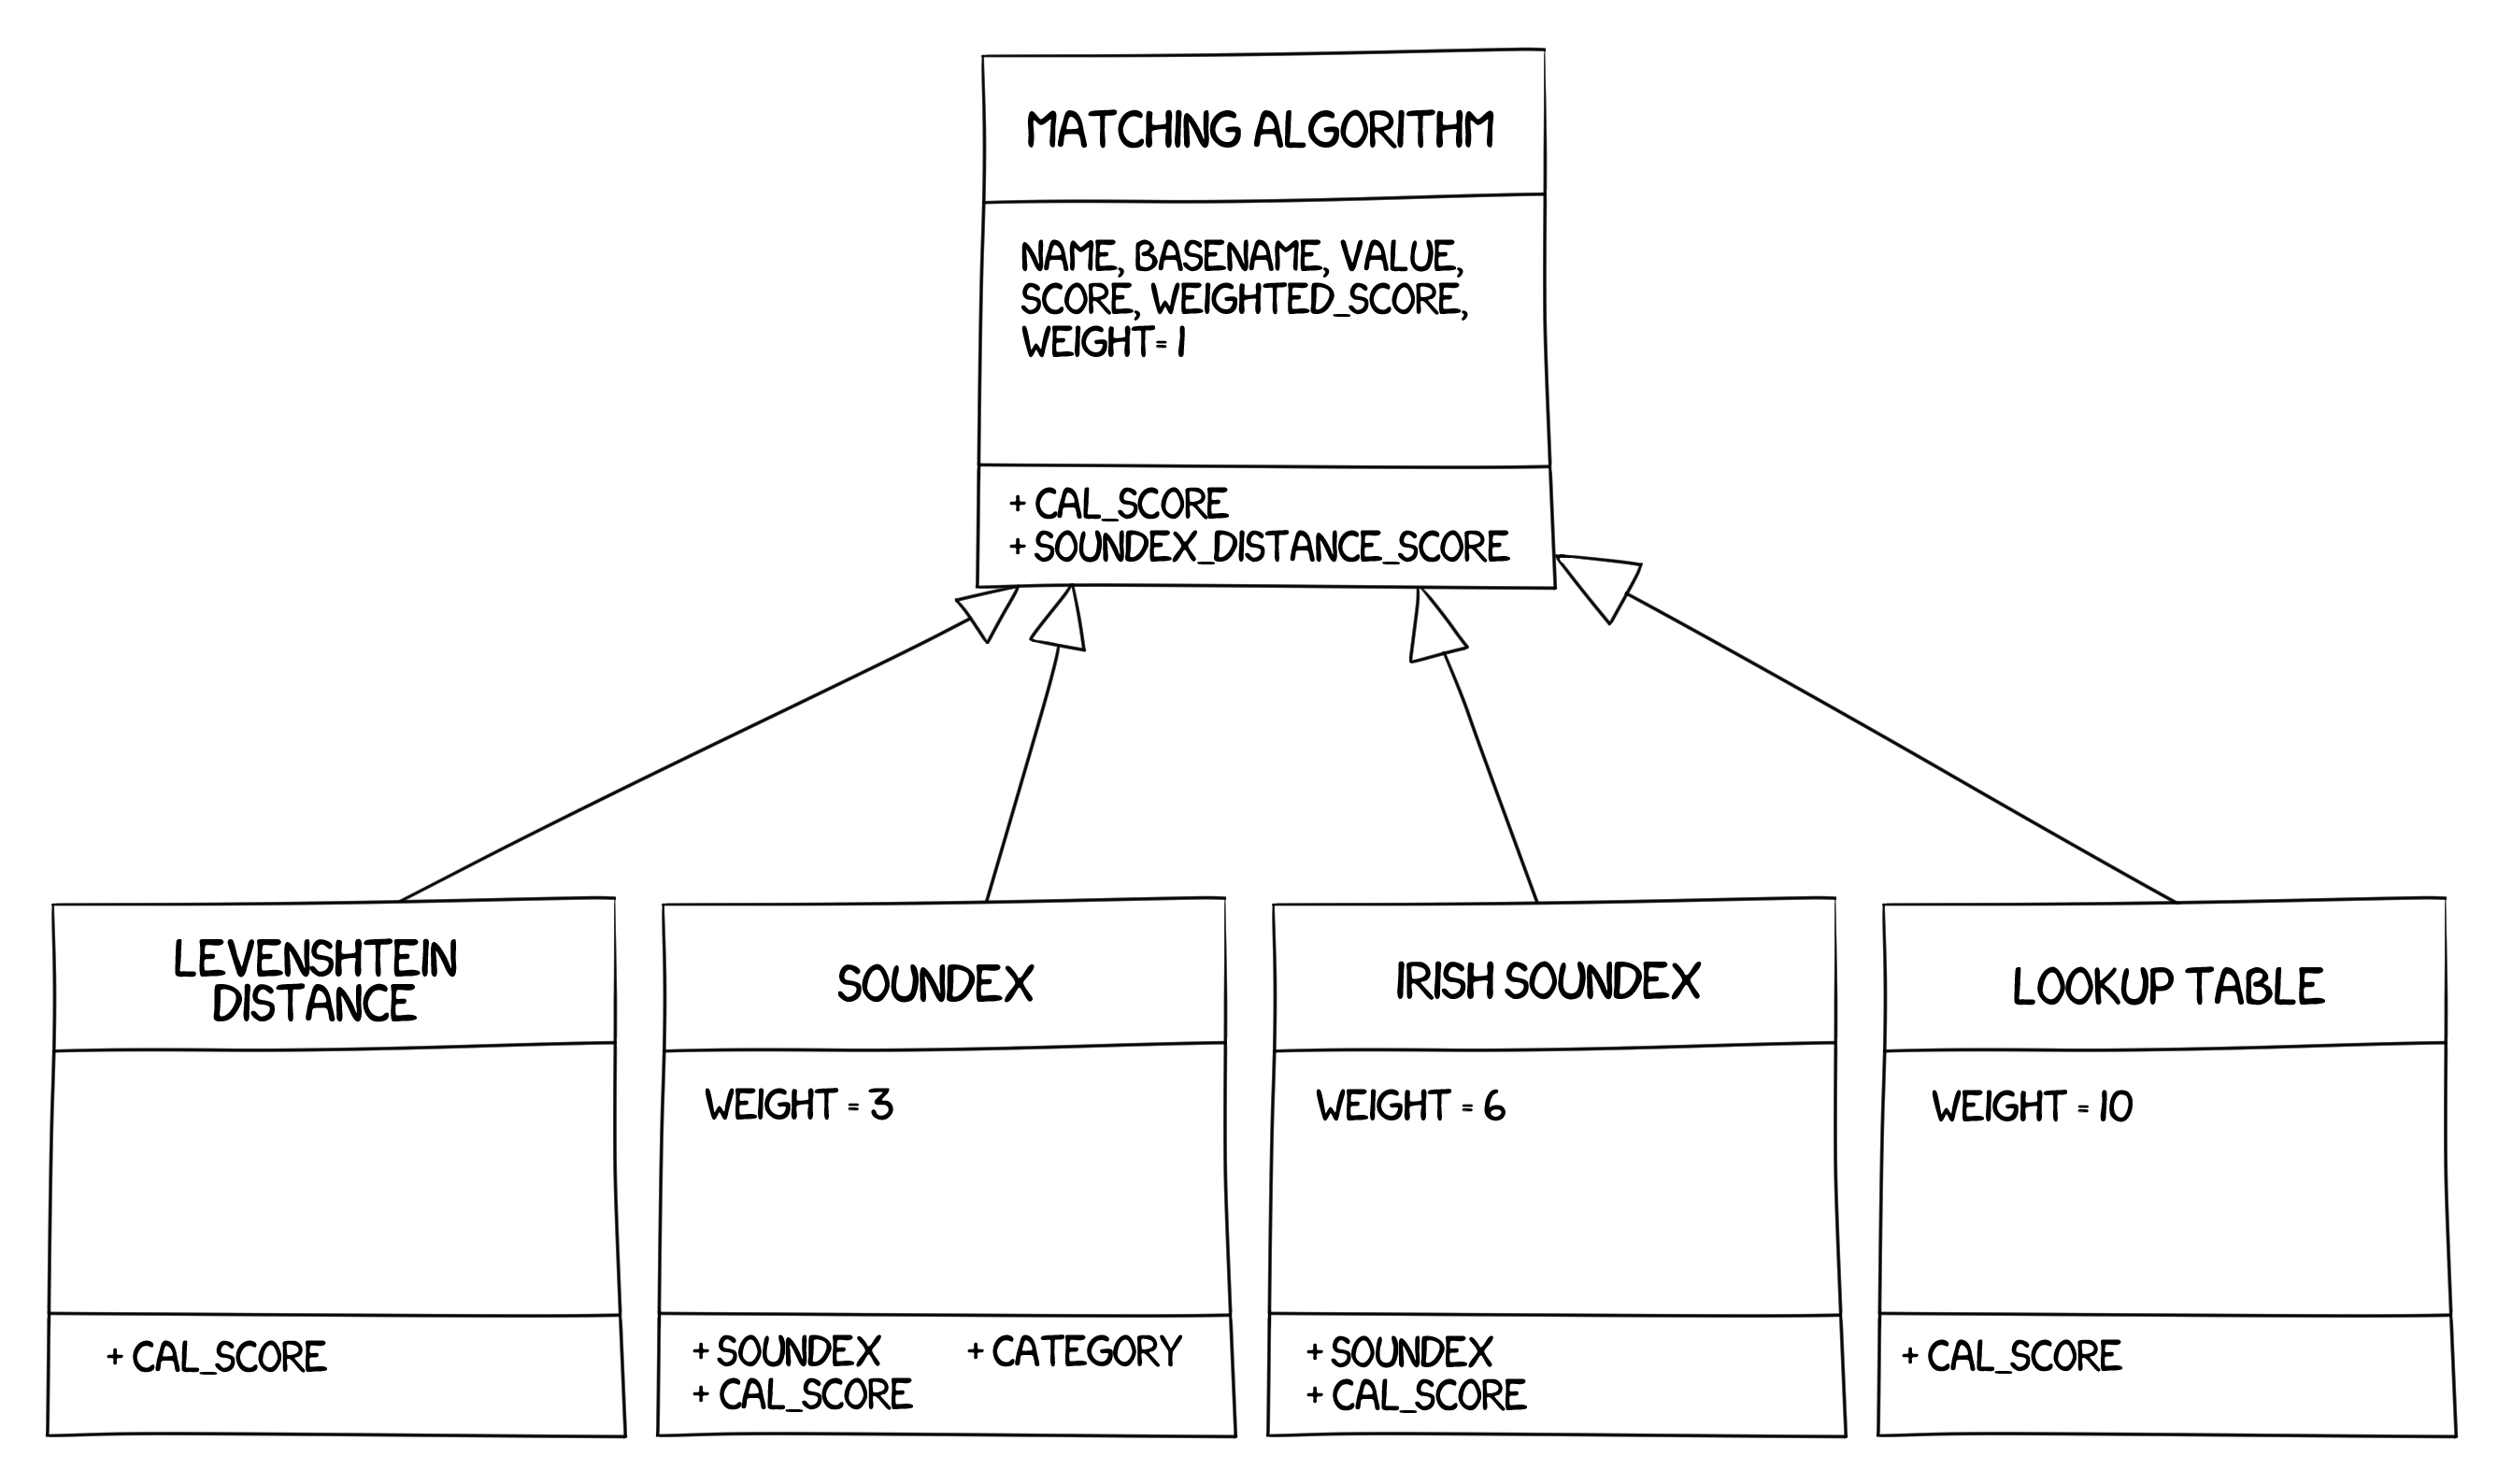
\includegraphics[width=16cm]{gfx/matching_inheritance_i}}
\caption{\texttt{MatchingAlgorithm} inheritance.}
\label{fig:mai}
\end{figure}

All matching algorithms (chapter \ref{ch:nma}) inherit the same superclass,\\
\texttt{MatchingAlgorithm} (shown in figure \ref{fig:mai} and
listing \ref{lst:ma_imp}). They all use the same class constructor
(in Ruby, it is called the \emph{initialize} method). To create an instance
of \texttt{MatchingAlgorithm}, current \emph{base name}, \emph{to-match name}
and \emph{weight} are passed as parameters.

We use \emph{The Strategy Pattern}\footnote{\cite[]{hf}, page 24}
as a design pattern. In \texttt{MatchingAlgorithm} the \texttt{cal\_score} method
is declared and also meant to be overridden, so every matching
algorithm needs to override this method using their own matching logic.
Each matching algorithm class will call \texttt{cal\_score}
to calculate its scores.
\texttt{cal\_score} is also private to be only used within the subclasses
themselves.

We also define \texttt{soundex\_distance\_score} method to be shared
between soundex algorithms. Any further shared methods can be declare
here as well.

\texttt{MatchingAlgorithm} class is shown in listing \ref{lst:ma_imp}.

\begin{minipage}{\linewidth}
\begin{lstlisting}[label={lst:ma_imp}, caption={\texttt{MatchingAlgorithm} class.}]
class MatchingAlgorithm
  WEIGHT = 1  # Default weight of every matching algorithm.

  attr_accessor :name,
    :base_name,
    :value,
    :label,
    :score,
    :weight,
    :weighted_score

  def initialize(params = {})
    @name      = params.fetch(:name)
    @base_name = params.fetch(:base_name)
    @weight    = params.fetch(:weight)

    cal_score
    @score = @score.round(3)
    @weighted_score = (@score * @weight).round(3)
  end

  private

  def cal_score
    raise NotImplementedError
  end

  def soundex_distance_score(s1, s2)
    if s1.first != s2.first
      0  # Different category, so they suppose to be completely different
    else
      (s1.size - Text::Levenshtein.distance(s1, s2).to_f ) / s1.size
    end
  end
end
\end{lstlisting}
\end{minipage}

For example of a concrete matching algorithm,
we have already shown some \texttt{cal\_score} overridings. For
\emph{Levenshtein distance} is as in in listing \ref{lst:leven}.
Here we will show whole \texttt{LevenshteinDistance} class,
which is a subclass of \texttt{MatchingAlgorithm}, as in listing \ref{lst:leven_class}.

\begin{minipage}{\linewidth}
\begin{lstlisting}[label={lst:leven_class}, caption={\texttt{LevenshteinDistance} class.}]
class LevenshteinDistance < MatchingAlgorithm
  private

  def cal_score
    @value = Text::Levenshtein.distance(@name, @base_name.name)
    size   = [@name.size, @base_name.name.size].max
    @score = ((size - @value).to_f / size)
  end
end
\end{lstlisting}
\end{minipage}

Also for \emph{Lookup table} is as in listing \ref{lst:lookup}.
Here we will show whole \texttt{LookupTable} class,
which is another subclass of \texttt{MatchingAlgorithm}, as in listing \ref{lst:leven_class}.
Note that \texttt{LookupTable} overrides default \emph{weight}, which
\texttt{LevenshteinDistance} does not.

\begin{minipage}{\linewidth}
\begin{lstlisting}[label={lst:lt_class}, caption={\texttt{LookupTable} class.}]
class LookupTable < MatchingAlgorithm
  WEIGHT = 10  # Overriding default weight.

  private

  def cal_score
    ...
  end
end
\end{lstlisting}
\end{minipage}

\section{Exporting a class method}

When we mentioned soundex implementation in listing \ref{lst:soundex},
we introduced \texttt{self.soundex} method instead of \texttt{cal\_score}.
Defining a method with \texttt{self.} is to create a \emph{class method} \cite[]{classmethod}.
\emph{Class method} can be called directly without creating instance of the class,
it is the same as \emph{static method} in Java. For example as in listing
\ref{lst:classmethod}.

\begin{minipage}{\linewidth}
\begin{lstlisting}[label={lst:classmethod}, caption={Calling class method \emph{Soundex.soundex}.}]
[7] pry(main)> Soundex.soundex('SMITH')
=> "S530"
\end{lstlisting}
\end{minipage}

By defining this method to be a \emph{class method}, it can be reused
in other class as well. In listing \ref{lst:sd_class} we will show whole
\texttt{Soundex} class, which is another subclass of \texttt{MatchingAlgorithm}.

\begin{minipage}{\linewidth}
\begin{lstlisting}[label={lst:sd_class}, caption={\texttt{Soundex} class.}]
class Soundex < MatchingAlgorithm
  WEIGHT = 3

  def self.soundex(name)
    ...
  end

  private

  def self.category(c)
    ...
  end

  def cal_score
    name_soundex      = self.class.soundex(@name)
    base_name_soundex = self.class.soundex(@base_name.name)

    @value = "#{base_name_soundex} <=> #{name_soundex}"
    @score = soundex_distance_score(name_soundex, base_name_soundex)
  end
end
\end{lstlisting}
\end{minipage}

Note that we have already covered \texttt{self.soundex} and \texttt{self.category} implementation
in listing \ref{lst:soundex} and \ref{lst:soundexc} respectively, so both
are truncated for readability. Here we focus on the \texttt{cal\_score} overriding
on \texttt{Soundex} class. The use of \texttt{self.class.soundex} in \texttt{cal\_score}
refers to \texttt{Soundex.soundex}. And \texttt{soundex\_distance\_score}
is defined in \texttt{MatchingAlgorithm}.

As for Irish soundex, it also contains its own \texttt{self.soundex}
\emph{class method}. But this \texttt{self.soundex} also calls \texttt{Soundex.soundex}
to use original soundex code, as in listing \ref{lst:is_call_s} (extracted from
\texttt{IrishSoundex.soundex} implementation, listing \ref{lst:irishsoundex}).

\begin{minipage}{\linewidth}
\begin{lstlisting}[label={lst:is_call_s}, caption={\texttt{IrishSoundex.soundex} calls to \texttt{Soundex.soundex}.}]
# Call to traditional soundex.
return {
  :label => name,
  :soundex => Soundex.soundex(name)
}
\end{lstlisting}
\end{minipage}

In listing \ref{lst:is_class} we will show whole \texttt{IrishSoundex} class,
which is another subclass of \texttt{MatchingAlgorithm}.

\begin{minipage}{\linewidth}
  \begin{lstlisting}[label={lst:is_class}, caption={\texttt{IrishSoundex} class.}]
class IrishSoundex < MatchingAlgorithm
  WEIGHT = 6

  def self.soundex(name)
    ..
  end

  private

  def cal_score
    name_soundex      = self.class.soundex(@name)
    base_name_soundex = self.class.soundex(@base_name.name)

    @value = "#{base_name_soundex[:soundex]} <=> #{name_soundex[:soundex]}"
    @label = name_soundex[:label]
    @score = soundex_distance_score(name_soundex[:soundex], base_name_soundex[:soundex])
  end
end
\end{lstlisting}
\end{minipage}

Note that we have already covered \texttt{self.soundex} implementation
in listing \ref{lst:irishsoundex}, so it is truncated for readability.
Here we focus on the \texttt{cal\_score} overriding
on \texttt{IrishSoundex} class. The use of \texttt{self.class.soundex} in \texttt{cal\_score}
refers to \texttt{IrishSoundex.soundex}. And \texttt{soundex\_distance\_score}
is defined in \texttt{MatchingAlgorithm}.

\section{Implementing new matching algorithms}

Currently there are 4 matching algorithms derived from
\texttt{MatchingAlgorithm}.

\begin{enumerate}
  \item \texttt{LevenshteinDistance}
  \item \texttt{Soundex}
  \item \texttt{IrishSoundex}
  \item \texttt{LookupTable}
\end{enumerate}

The implementations of all of these classes are within the same file
as their superclass, \texttt{MatchingAlgorithm}, the path is\\
\texttt{app/models/matching\_algorithm.rb}. The structure of this file
is shown in listing \ref{lst:maf}.

\begin{minipage}{\linewidth}
  \begin{lstlisting}[label={lst:maf}, caption={\texttt{matching\_algorithm.rb}.}]
class MatchingAlgorithm
  ..
end

class LevenshteinDistance < MatchingAlgorithm
  ..
end

class Soundex < MatchingAlgorithm
  ..
end

class IrishSoundex < MatchingAlgorithm
  ..
end

class LookupTable < MatchingAlgorithm
  ..
end
\end{lstlisting}
\end{minipage}

To add a new matching algorithm, suppose we were to implement another
soundex for Indian \cite[]{indiansoundex}. We would call this \texttt{IndianSoundex}.
Here is the list of steps to do so.

\begin{enumerate}
  \item Modify the file \texttt{app/models/matching\_algorithm.rb} where all
    the matching algorithms are in. Append the class definition to the file.

    \begin{minipage}{\linewidth}
    \begin{lstlisting}
..

class LookupTable < MatchingAlgorithm
  ..
end

class IndianSoundex < MatchingAlgorithm
  private

  def cal_score
    # To be implemented.
  end
end
    \end{lstlisting}
    \end{minipage}

  \item Override \texttt{cal\_score}, fulfil the algorithm for Indian
    soundex.
  \item You may create \emph{class method} \texttt{self.soundex} to follow
    the same pattern as \texttt{Soundex} and \texttt{IrishSoundex}, making
    it reusable too.
  \item You may also use \emph{class method} of soundex and Irish soundex
    by calling to \texttt{Soundex.soundex} and \texttt{IrishSoundex.soundex}.
  \item You may also use shared method \texttt{soundex\_distance\_score}
    to calculate distance score like two other soundexes do.
\end{enumerate}

You may consider adding more shared methods to \texttt{MatchingAlgorithm}
superclass if considered appropriate, i.e. many subclasses will use it.
On the other hand, if you need some method just inside the class,
consider create just private methods.

